%!TEX root=paper.tex

% \newpage
\subsection{Practicing Personalized Vocabulary in Context}

% Given the list of words that a user looked up -- and are thus likely to be unknown -- we can generate exercises for them. 
Given that the translation API captures the context together with every translation, exercises can be personalized for every user based on their past reading by using the original context in which the words have been encountered.

Figure \ref{fig:exercise_translate} shows such a generated exercise which asks the reader to translate a given word in the context in which it was encountered in a past reading. The main interactive elements (IEs) that are specific to this exercise are an input box that allows the user to enter a solution (IE5); a button for checking the correctness of the input answer (IE2); a hint button which presents the correct answer (IE1). Two types of control that span exercise types are: a word pronunciation option (IE3) and a feedback option (IE4) which allows the user to provide feedback about the exercise.

\begin{figure}[h!]
\centering
  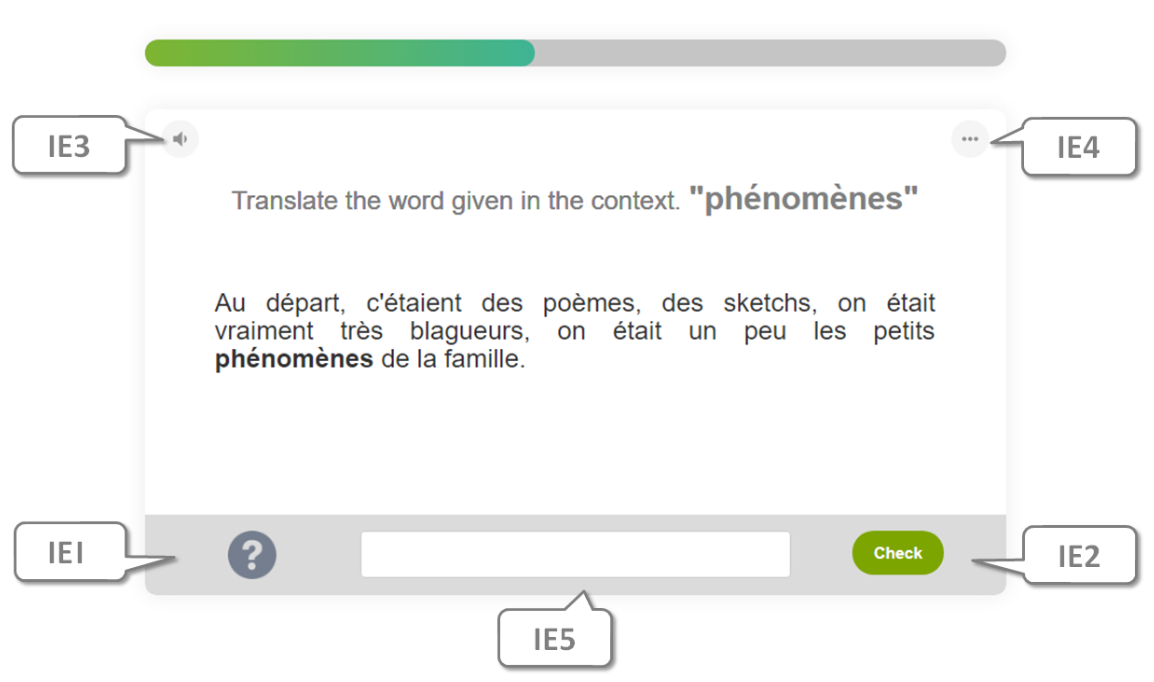
\includegraphics[width=0.9\columnwidth]{figures/exercise_translate}
  \caption{Translate exercises ask the user to translate a word in a given context (retrieved from the user's past readings)}
  \label{fig:exercise_translate}
\end{figure}

	The system currently implements three other types of vocabulary practice exercises\footnote{Detailed description of the exercise types are elsewhere\cite{Avagyan17a-blocks}}, which can be split into two categories: 
\begin{enumerate}
	
	\item Free text input -- where the text must be typed in the learned language (exercise type: Find)

	\item Multiple choice -- where the user is presented with a set of alternatives (exercise types: Choose, and Match). 

\end{enumerate}

% \subsubsection{Selecting Words to Study}

Since a learner might encounter many words that are not understood, we need to prioritize those that are to be studied in exercises. We use two aspects to prioritize words: 

% The words good for study are the ones that are either starred by the user, or are important and of quality based on a set of heuristics. 

\begin{enumerate}

  \item Word Importance. The system prioritizes words based on the frequency with which they appear in the language.\footnote{For word frequencies we use frequencies computed based on movie subtitles which have been shown to be highly representative to frequencies in human interacitons \cite{New07-subtitles}}. 
  
  \item Context Quality. The system favors words that come with a context which is not too short but not too long. 

\end{enumerate}

